\begin{figure}[t]
\centering
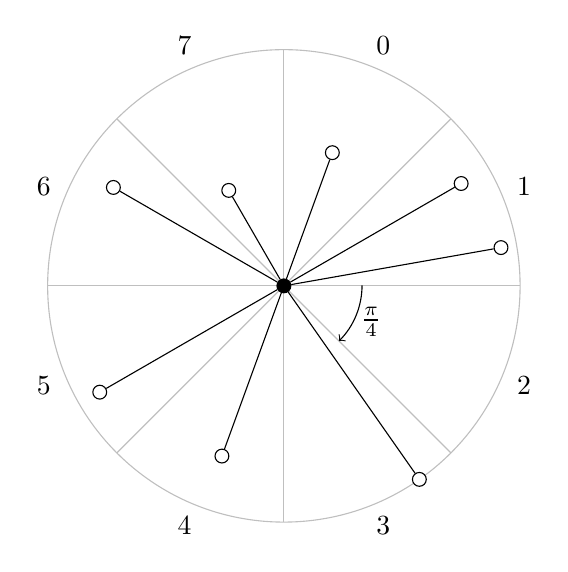
\begin{tikzpicture}
  % Kreis.
  \draw[color=lightgray] (0, 0) circle (3);

  % Partitionsbeschriftungen
  \node (2) at (22.5:3.3) {$1$};
  \node (1) at (67.5:3.3) {$0$};
  \node (8) at (112.5:3.3) {$7$};
  \node (7) at (157.5:3.3) {$6$};
  \node (6) at (202.5:3.3) {$5$};
  \node (5) at (247.5:3.3) {$4$};
  \node (4) at (292.5:3.3) {$3$};
  \node (3) at (337.5:3.3) {$2$};

  % Partitionierungen.
  \draw[color=lightgray] (0, 0) -- (0:3);
  \draw[color=lightgray] (0, 0) -- (45:3);
  \draw[color=lightgray] (0, 0) -- (90:3);
  \draw[color=lightgray] (0, 0) -- (135:3);
  \draw[color=lightgray] (0, 0) -- (180:3);
  \draw[color=lightgray] (0, 0) -- (225:3);
  \draw[color=lightgray] (0, 0) -- (270:3);
  \draw[color=lightgray] (0, 0) -- (315:3);

  % Graph.
  \tikzstyle{node}=[circle,draw, minimum width=5pt, inner sep=0pt, fill=white]
  \tikzstyle{root}=[fill=black]

  \node[node, root] (root) at (0,0) {};
  \node[node] (a) at (10:2.8) {};
  \node[node] (b) at (30:2.6) {};
  \node[node] (c) at (70:1.8) {};
  \node[node] (d) at (120:1.4) {};
  \node[node] (e) at (150:2.5) {};
  \node[node] (f) at (210:2.7) {};
  \node[node] (g) at (250:2.3) {};
  \node[node] (h) at (305:3) {};

  \path (root) edge (a);
  \path (root) edge (b);
  \path (root) edge (c);
  \path (root) edge (d);
  \path (root) edge (e);
  \path (root) edge (f);
  \path (root) edge (g);
  \path (root) edge (h);

  % Winkel.
  \draw[<-] (0.7, -0.7) arc (-45:0:1);
  \node[] at (-22.5:1.2) {$\frac{\pi}{4}$};
\end{tikzpicture}
\caption[Partitionierung eines Graphknotens]{Partitionierung eines Graphknotens im Uhrzeigersinn in $P = 8$ Bereiche mit gleichmäßigen Innenwinkeln der Größe $\pi/4$.}
\label{fig:partitionierung}
\end{figure}
